\documentclass{article}

\usepackage{ScientificColourMapsTikz/batlow}
\usepackage{arealegendstyle}
\pgfplotsset{compat=1.18}

\title{Test Colourmaps}
\author{Til Gärtner}

\begin{document}

\maketitle

\centering
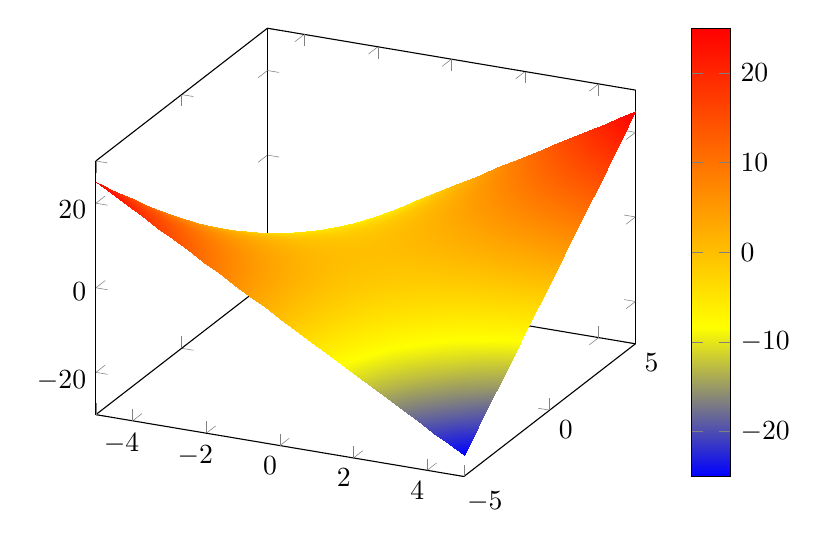
\begin{tikzpicture}
    \begin{axis}[colorbar]
        \addplot3[surf, shader=interp] {x*y};
    \end{axis}
\end{tikzpicture}

\begin{tikzpicture}
    \begin{axis}[colormap name=batlow10, colorbar, colorbar sampled, colorbar style={samples=11}]
        \addplot3[surf, shader=flat, colormap access=const] {x*y};
    \end{axis}
\end{tikzpicture}

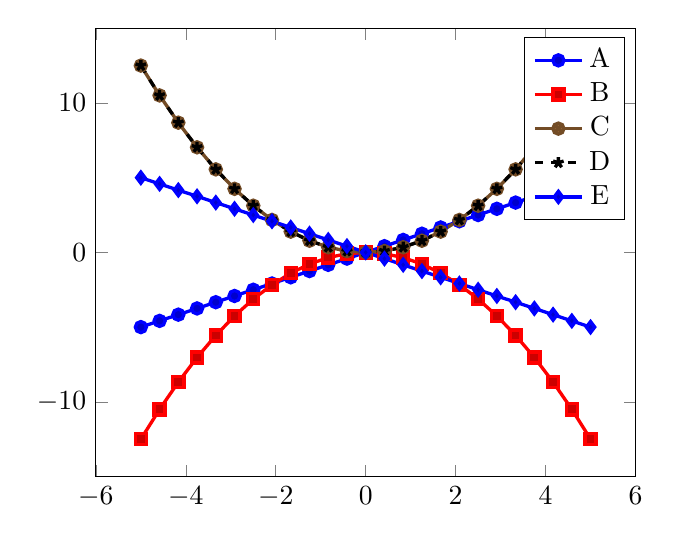
\begin{tikzpicture}
    \begin{axis}
        \addplot+[very thick] {x};
        \addplot+[very thick] {-x*x/2};
        \addplot+[very thick] {x*x/2};
        \addplot+[very thick, dashed] {x*x/2};
        \addplot+[very thick] {-x};

        \addlegendentry{A}
        \addlegendentry{B}
        \addlegendentry{C}
        \addlegendentry{D}
        \addlegendentry{E}
    \end{axis}
\end{tikzpicture}

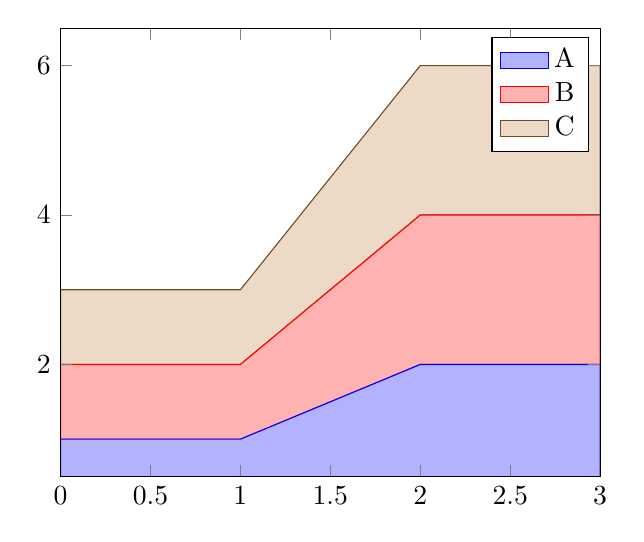
\begin{tikzpicture}
    \begin{axis}[
        stack plots=y,
        area style,
        enlarge x limits=false,
    ]
        \addplot coordinates
            {(0,1) (1,1) (2,2) (3,2)}
                \closedcycle;
        \addplot coordinates
            {(0,1) (1,1) (2,2) (3,2)}
                \closedcycle;
        \addplot coordinates
            {(0,1) (1,1) (2,2) (3,2)}
                \closedcycle;
        
        \addlegendentry{A}
        \addlegendentry{B}
        \addlegendentry{C}
    \end{axis}
\end{tikzpicture} 

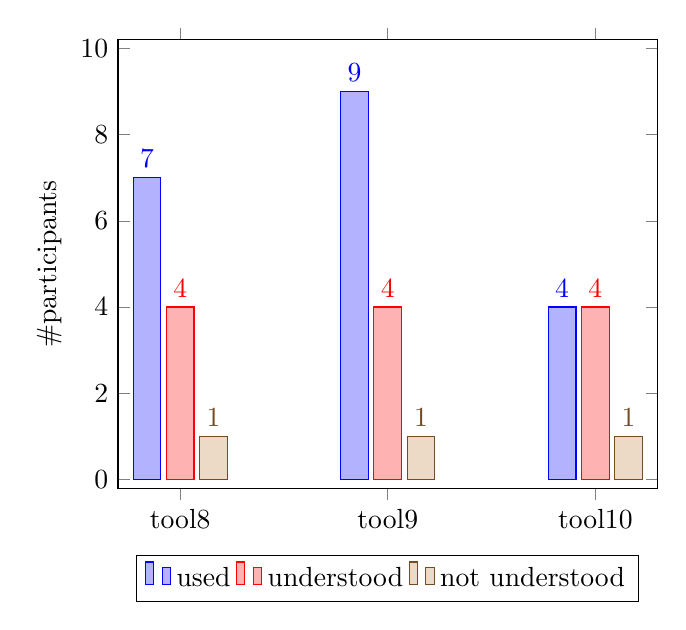
\begin{tikzpicture}
    \begin{axis}[
        ybar,
        enlargelimits=0.15,
        legend style={at={(0.5,-0.15)},
        anchor=north,legend columns=-1},
        ylabel={\#participants},
        symbolic x coords={tool8,tool9,tool10},
        xtick=data,
        nodes near coords,
        nodes near coords align={vertical},
    ]
        \addplot coordinates {(tool8,7) (tool9,9) (tool10,4)};
        \addplot coordinates {(tool8,4) (tool9,4) (tool10,4)};
        \addplot coordinates {(tool8,1) (tool9,1) (tool10,1)};
        \legend{used,understood,not understood}
    \end{axis}
\end{tikzpicture} 

\end{document}
